%!TEX root = ../thesis.tex

% **************************** Define Graphics Path **************************
\ifpdf
    \graphicspath{{Chapter4/Figs/Raster/}{Chapter4/Figs/PDF/}{Chapter4/Figs/}{Chapter4/}}
\else
    \graphicspath{{Chapter4/Figs/Vector/}{Chapter4/Figs/}{Chapter4/}}
\fi


\chapter{Quantum Metropolis Sampling Revived}
\label{chapter:quantum_metropolis}
\section{Introduction}
Sampling thermal (Gibbs) states of physical systems is one of the most credible applications for future fault-tolerant quantum computers. Thermal expectation values are of interest across quantum chemistry, condensed matter physics and high energy physics, and classically they are almost all computed by Markov chain Monte Carlo. For many fermionic or frustrated spin systems this approach runs into the sign problem as the weights are not all positive. As the average sign decays exponentially with system size and inverse temperature, the number of samples necessary to resolve the observable grows exponentially \cite{Troyer_2005}. A quantum computer can directly interact with the state rather than only with a signed decomposition, so it does not encounter the sign problem. The classical computer is attempting to replicate the interference that physics gives for free on a quantum computer.

The original quantum algorithm invented for performing this sampling was the Quantum Metropolis algorithm of Temme et. al. \cite{Temme_2011}. This was a direct quantum analogue of Metropolis-Hastings: propose a random unitary move then accept or reject the move based upon the energy before and after the move. The principal challenge of creating a quantum analogue of the Metropolis-Hastings algorithm was rejecting a move. In the classical setting one can either copy the state before the move or simply undo the move after rejecting, however, in the quantum setting copying the initial state is forbidden by the no-cloning principle and simply reversing the proposed unitary does not undo the disturbance caused by the accept/reject measurement. Temme et. al. \cite{Temme_2011} navigated around these challenges by using a Marriott-Watrous \cite{MarriottWatrous} inspired rewinding procedure to approximately return the system to its previous energy upon rejecting a move.

The rewinding procedure requires a modified quantum phase estimation (QPE) protocol, which harnesses the Fourier transform to coherently encode an estimate of the system’s energy in an ancilla register (Chapter~\ref{chapter:boosting_qpe}). This register is reused without resetting it during rewinding, hence the protocol must work even when the register is not initialised to $\ket{0}$. The original construction therefore required QPE to be ``shift-invariant": starting from a register value $p$ rather than zero simply translates the output by $p$. It also required ``boosting" to suppress the tails of the energy-estimation amplitudes that arise from this Fourier transform, reducing the weight of estimates far from the true energy. Thus, the original Quantum Metropolis algorithm depended upon a  ``boosted shift-invariant" quantum phase estimation protocol that applied a shift to an ancilla register within a given bound of the true energy (with $\tilde E_j = \frac{N}{2\pi}E_j$ with $N=2^{\eta}$ for an $\eta$ ancilla energy register):
\begin{equation}
  \ket{\psi_j}\ket{p} \;\mapsto\; \sum_{s} \alpha(E_j,s)\,\ket{\psi_j}\ket{p+s},
  \qquad\alpha(E_j,s) = 0 \ \text{ for } |s-\tilde E_j|_{N} > \mu .
  \label{eq:Boostedshiftinvariantqpe}
\end{equation}
where $\ket{\psi_j}$ is an energy eigenstates with energy $E_j$, $\mu$ is the allowed error in register units, and $|\cdot|_{N}$ measures distance accounting for the register’s wraparound.

Recently the field has been reshaped by a new paradigm based on Davies-generator Lindbladian evolution \cite{chen2023quantumthermalstatepreparation,Kastoryano2014QuantumGS,shtanko2021preparing,chen2021fast,chen2023efficient,rall2023thermal,gilyen2024quantum,ding2025efficient,ding2025end,guo2025designing,chen2025efficient, hahn2026efficient, scandi2026thermalization,leng2026accelerating,rouze2026optimal,lloyd2026quantum,Rouz__2026} which has largely displaced the Metropolis approach in the literature. This current dominance of Lindbaldian samplers is in no small part due to the no-go theorem contained in Appendix H of \cite{chen2023quantumthermalstatepreparation}. This proved it is impossible to implement the ``boosted shift-invariant" quantum phase estimation protocol \eqref{eq:Boostedshiftinvariantqpe} that the original Quantum Metropolis algorithm required.  The original implementation \cite{Temme_2011} suggested taking the median of multiple QPE runs which fails to be ``shift-invariant" as the difference of medians is not necessarily close to the median of the differences. This no-go theorem is widely regarded as closing the book on Quantum Metropolis sampling. 

In this chapter we restore the Quantum Metropolis algorithm by harnessing the Boosted State-Independent Quantum Phase Estimation (BSI-QPE) protocol of Section~\ref{section:boostedphaseestimation} to navigate around this no-go theorem. In Chapter~\ref{chapter:boosting_qpe} the Fourier transform turned the problem of boosting QPE into a problem of designing window functions, and by designing a novel complementary pair of window functions we obtained a protocol which ensures the magnitude of the shift in the ancilla register is close to the true energy with the sign of this shift recorded in an additional flag qubit (Eq.~\eqref{eq:bsi_qpe}). This protocol is implementable and can fulfill the same role as the previous impossible protocol, with the modification that whenever we previously controlled off the value of the energy register we now must also control off the flag qubit. We carefully account for the non-zero but exponentially suppressed tails of this protocol in our proof work.

Our main contributions are as follows:
\begin{enumerate}
    \item \textbf{Harnessing BSI-QPE} (Sections~\ref{section:band_limited_bsiqpe} and~\ref{section:algorithm}): We modify the Quantum Metropolis algorithm to utilise BSI-QPE, controlling off the flag qubit wherever we previously controlled off the energy register. We show that BSI-QPE is close in operator norm to a fully band-limited protocol, and that unboosted QPE is insufficient for our later proof of approximate quantum detailed balance without a promise that energies are exactly representable in $\eta$ bits.
    \item \textbf{Elementary analysis of rewinding} (Section~\ref{section:rejection}): We provide an alternative explanation of the rewinding procedure to the Jordan's-lemma treatment of \cite{Temme_2011} which we find more transparent.
    \item \textbf{Approximate Quantum Detailed Balance Condition} (Section~\ref{section:detailedbalancedef}): We introduce a new branch-wise KMS-inspired detailed balance criteria. This allows us to consider the additive errors introduced by the exponentially suppressed (but non-zero) tails of our BSI-QPE protocol that were neglected in the original treatment \cite{Temme_2011}. We later use this condition to establish that the algorithm approximately preserves the Gibbs state.
    \item \textbf{Approximate Quantum Detailed Balance Proof} (Section~\ref{section:proofmain}): We introduce a novel \textbf{truncate} step to the proof which bounds the additive error due to the non-zero tails of BSI-QPE. We carefully convert the modular norm of the energy approximations to a standard norm \eqref{eq:condJ}-\eqref{eq:kappaclose}. We provide a novel and elegant proof (Lemma~\ref{lemma:summed-history-reversal}) that the measurement outcomes during the rejection procedure can be reversed. Further, we derive an error term \eqref{eq:Wdrifterror} overlooked in \cite{Temme_2011} that is due to the QPE energy register not being exactly returned to $\ket{0}$.
    \item \textbf{Main result} (Theorem~\ref{theorem:main}): Let $\mathcal{E}$ be one  update step of the Quantum Metropolis algorithm run with $\eta$ ancilla qubits in the energy register and a budget of at most $n^*$ rewinding attempts. Under the conditions of Theorem 1, the fixed point $\sigma^*$ of $\mathcal{E}$ is close to the Gibbs state $\sigma_G$ in trace norm $\|\cdot\|_*$:
    \begin{equation}
       \|\sigma_G- \sigma^*\|_* = O\left(\frac{\ell\max\left( n^{*\frac{7}{2}}\sqrt{\frac{\beta\|H\| }{2^{\eta}}}\log^{\frac{9}{2}}n^*,\frac{1}{n^*}\right)}{1-k}\right)
    \end{equation}
    where $k$ is the ergodicity coefficient of $\mathcal{E}^\ell$.
\end{enumerate}
Theorem~\ref{theorem:main} restores the approximate Gibbs-invariance result of the original framework \cite{Temme_2011}, as before this does not directly prove rapid convergence which depends on the mixing properties of $\mathcal{E}$. Proving polynomial time convergence for a general Hamiltonian is likely infeasible as it would allow the solution of QMA-complete problems in polynomial time \cite{kempe2006complexity}. However, under the assumption of strict trace-norm contractivity taken in \cite{Temme_2011} we prove exponentially fast convergence to the fixed point.

Three other routes to Metropolis-type dynamics sidestep shift-invariant phase estimation entirely. Jiang and Irani \cite{jiang2024quantummetropolissamplingweak} replace rewinding with weak measurement and prove that the Gibbs state is an approximate fixed point. Because each iteration moves the state only by $O(\tau^2)$ for a small weak-measurement parameter $\tau$, the number of iterations grows by a polynomial factor. Zhang, Bosse and Cubitt \cite{zhang2023dissipative} instead weakly measure the local terms of the Hamiltonian in sequence with the Gibbs state reached at the stopping time of a conditionally stopped process rather than as the fixed point of a Markov chain. Gilyén et al. \cite{gilyen2024quantum} construct efficiently implementable discrete-time channels that are exactly detailed balanced. They also show how Metropolis-style samplers that estimate energies before and after a jump can be made exactly detailed balanced, implementing rejection with an additional Kraus operator rather than by Marriott–Watrous rewinding. Our guarantees are weaker than those of \cite{gilyen2024quantum}: we obtain approximate rather than exact Gibbs stationarity, and we prove no mixing-time bounds. Our contribution is of a different kind. We show that the original accept/reject-with-rewinding architecture of \cite{Temme_2011}, widely regarded as ruled out, is sound, because it requires a weaker phase-estimation primitive than the one the no-go theorem \cite{chen2023quantumthermalstatepreparation} forbids. We regard these frameworks as complementary, and which is most efficient in practice remains open.

The remainder of this chapter is organised as follows. Section~\ref{section:band_limited_bsiqpe} bounds the error from truncating the tails of BSI-QPE and explains why boosting is necessary. Section \ref{section:algorithm} describes our modified Quantum Metropolis algorithm incorporating BSI-QPE; Fig.~\ref{fig:quantum-metropolis-flowchart} provides an complete overview to help guide the reader. Section~\ref{section:why} presents the main theorem of this chapter, defines our approximate quantum detailed balance framework, and outlines the four-step proof strategy applied to each branch; the full proofs are given in Appendices~\ref{appendix:Aproof} and \ref{appendix:Bproof}. Finally, Section \ref{section:discussion} discusses the broader implications of our results, the assumptions made, and the outlook for implementing these techniques on near-term or fault-tolerant quantum hardware.



\section{Band-limited BSI-QPE}
\label{section:band_limited_bsiqpe}
The window functions $\alpha(x) = \text{sech}( r\cos^{2b} \frac{\pi x}{N})$ and $\beta(x) = \text{tanh}(r \cos^{2b} \frac{\pi x}{N})$ of Section~\ref{section:appendix} both have discrete Fourier transforms which decay exponentially fast:
\begin{equation}
    |\hat \alpha(k)|,|\hat \beta(k)| = O\left( \frac{1}{\nu}e^{-\nu |k|}\right)
    \label{eq:scaling}
\end{equation}
where $\nu = \frac{1}{2b}$. Hence we can write:
\begin{equation}
    \hat\alpha(k) = \tilde\alpha(k) + \Delta_{\alpha}(k) \>\>\>\>\>\>\hat\beta(k) = \tilde\beta(k) + \Delta_{\beta}(k)
    \label{eq:decomposealpha}
\end{equation}
where:
\begin{align}
    \tilde\alpha(k) &= \hat\alpha(k)\mathbbm{1}(|k|_{N}\leq \mu)\\
    \tilde\beta(k) &= \hat\beta(k)\mathbbm{1}(|k|_{N}\leq \mu)
    \label{eq:decomposealpha2}
\end{align}  and
\begin{equation}
    \sum_k|\Delta_\alpha(k)|,\sum_k|\Delta_\beta(k)|\leq \epsilon_{\Delta}
    \label{eq:decomposealpha3}
\end{equation} where $\epsilon_{\Delta} = O(\frac{1}{\nu}e^{-\nu \mu})$ and $|x|_N = \min(x \mod N,- x\mod N)$ is the modular norm value of $x$.

\begin{lemma}[Band-limited BSI-QPE]
\label{lemma:0}
    Define $\widetilde{\text{BSI-QPE}}$ as given by:
    \begin{equation}
       \widetilde{\text{BSI-QPE}}= \sum_j \sum_{p,q} \tilde G^{pq}_j \otimes \ket{p}\bra{q} \otimes \ket{\psi_j}\bra{\psi_j}
    \end{equation}
    where 
    \begin{equation}
        \tilde G^{pq}_j = \left(\begin{smallmatrix}
        (-1)^{q-p}\tilde\alpha(q-p+\frac{N}{2\pi}E_jt) && \tilde\beta(q-p+\frac{N}{2\pi}E_jt)\\
        -\tilde\beta (q-p-\frac{N}{2\pi}E_jt) && (-1)^{q-p}\tilde\alpha(q-p-\frac{N}{2\pi}E_jt)
    \end{smallmatrix}\right)
    \end{equation}
    Then,  
    \begin{equation}
        \|\widetilde{\text{BSI-QPE}}-\text{BSI-QPE}\| \leq 2\epsilon_{\Delta}
    \end{equation}
\end{lemma}
Proof is given in Appendix~\ref{section:appendixTrunc}. This shows that our BSI-QPE protocol is very close in operator norm to a fully band-limited BSI-QPE.

\begin{remark}[Why boosting is necessary]
Instead one could attempt to use unboosted state-independent QPE. This would correspond to choosing $\alpha(x)=1$, which simplifies Fig.~\ref{fig:circuit} to Fig.~\ref{fig:standard_qpe}. As this effectively acts as a rectangular window function, $|\hat\alpha(k)| = O(\frac{1}{k})$ for off-grid $k$, so $\epsilon_{\Delta} = O(\log \frac{N}{\mu})$ (compared to $\epsilon_{\Delta} = O(2^{-\nu \mu})$ for BSI-QPE). This bound exceeds $1$ and so unboosted state-independent QPE is insufficient for Quantum Metropolis sampling without the promise of energies exactly represented in $\eta$ bits.
\end{remark}

\subsection{Algorithm}
\label{section:algorithm}
Quantum metropolis is heavily inspired by the classical metropolis-hastings algorithm. The principal idea is to apply a randomly chosen update to the current state then accept/reject this update with a probability given by a function ($\tilde{f}_{E_aE_b}=\min(1, e^{-\beta(E_b-E_a)})$) of the energy before $(E_a)$ and after $(E_b)$ the update. This update process is repeated many times with the system quickly converging to equilibrium. To replicate this on a quantum computer we need to be able to: measure the energy of a state (Section~\ref{section:energymeasurement}), apply some update (Section~\ref{section:update}), accept/reject an update with the correct probability (Section~\ref{section:acceptprob}) and ``undo" an update upon deciding to reject it (Section~\ref{section:rejection}). Figure~\ref{fig:quantum-metropolis-flowchart} illustrates this full algorithm for a single update.


Throughout one full update, let $R$ denote the $\eta$-qubit BSI-QPE energy-index register and qubit $F$ the additional qubit on which the $G_j^{pq}$ act. At the start of the update, $R$ is initialised to $\ket{0}$ whilst $F$ is in the maximally mixed state (by classically choosing a random initial state $\ket{0}$ or $\ket{1}$) and the qubit $M$ on which the acceptance rotation $W_{abde}$ acts is initialized in $\ket{0}$. 
\begin{figure*}[t]
  \centering
  % Quantum Metropolis update: portrait, algorithm-at-a-glance flowchart.
% Required in the parent document:
%   \usepackage{amsmath,amssymb,tikz}
%   \usetikzlibrary{arrows.meta,backgrounds,fit,shapes.geometric}
%
% When a referenced label exists, \qmsectionref prints its section number.
% In a standalone build it falls back to the subsection title.
\makeatletter
\providecommand{\qmsectionref}[2]{%
  \ifcsname r@#1\endcsname Sec.~\ref{#1}\else\S~#2\fi}
\makeatother

\definecolor{qmNavy}{HTML}{17324D}
\definecolor{qmBlue}{HTML}{2F6B9A}
\definecolor{qmBlueFill}{HTML}{EAF3F8}
\definecolor{qmOrange}{HTML}{C66A1B}
\definecolor{qmOrangeFill}{HTML}{FFF2E6}
\definecolor{qmPurple}{HTML}{725A9A}
\definecolor{qmPurpleFill}{HTML}{F1EDF7}
\definecolor{qmGreen}{HTML}{2F7D5C}
\definecolor{qmGreenFill}{HTML}{E8F4EE}
\definecolor{qmRed}{HTML}{A33A3A}
\definecolor{qmRedFill}{HTML}{F9EAEA}
\definecolor{qmGray}{HTML}{52606D}
\definecolor{qmGrayFill}{HTML}{F4F6F8}

\begin{tikzpicture}[scale=.94,transform shape,
  font=\sffamily\footnotesize,
  line cap=round,
  line join=round,
  >={Stealth[length=2.4mm,width=1.7mm]},
  flow/.style={->,draw=qmNavy,line width=.9pt},
  process/.style={
    draw=qmNavy,fill=white,rounded corners=2.5pt,
    line width=.8pt,minimum height=10.5mm,minimum width=23mm,
    align=center,inner xsep=5pt,inner ysep=3.5pt
  },
  quantum/.style={process,draw=qmPurple,fill=qmPurpleFill},
  update/.style={process,draw=qmBlue,fill=qmBlueFill},
  test/.style={
    diamond,aspect=1.8,draw=qmNavy,fill=white,
    line width=.85pt,minimum width=20mm,minimum height=13mm,
    align=center,inner sep=1.5pt
  },
  state/.style={
    ellipse,draw=qmNavy,fill=qmGrayFill,line width=.85pt,
    minimum width=21mm,minimum height=10mm,align=center
  },
  accepted/.style={state,draw=qmGreen,fill=qmGreenFill},
  failed/.style={state,draw=qmRed,fill=qmRedFill},
  branchlabel/.style={
    font=\sffamily\scriptsize,fill=white,inner sep=1.5pt
  },
  stepref/.style={font=\sffamily\tiny,text=qmGray},
  note/.style={font=\sffamily\scriptsize,text=qmGray,align=center},
  legend/.style={
    draw=qmGray!55,fill=qmGrayFill,rounded corners=3pt,
    line width=.65pt,align=left,inner sep=6pt,
    text width=55mm,font=\sffamily\scriptsize
  }
]

% Main vertical spine -------------------------------------------------------
\node[state] (rho) at (0,0) {$\rho$};

\node[quantum] (energy) at (0,-1.65) {
  $E_{ae}$\\[-1pt]
  \scriptsize measure energy; record $(a,e)$\\[-1pt]
  \tiny\color{qmGray}\qmsectionref{section:energymeasurement}{Measure the energy}
};

\node[update] (chooseC) at (0,-3.35) {
  pick $C\sim\mathrm d\mu(C)$ and apply $C$\\[-1pt]
  \tiny\color{qmGray}\qmsectionref{section:update}{Update}
};

\node[quantum] (qpe) at (0,-5.05) {
  BSI--QPE\\[-1pt]
  \scriptsize prepare $(b,d)$ in the persistent $R,F$ register\\[-1pt]
  \tiny\color{qmGray}\qmsectionref{section:boostedphaseestimation}{Boosted phase estimation}
};

\node[quantum] (rotate) at (0,-6.75) {
  $W_{abde}$ on $M$\\[-1pt]
  \scriptsize acceptance rotation\\[-1pt]
  \tiny\color{qmGray}\qmsectionref{section:acceptprob}{Accept or Reject}
};

\node[test] (sdecision) at (0,-8.55) {
  measure $M$\\[-1pt]$s\ ?$
};

\draw[flow] (rho) -- (energy);
\draw[flow] (energy) -- (chooseC);
\draw[flow] (chooseC) -- (qpe);
\draw[flow] (qpe) -- (rotate);
\draw[flow] (rotate) -- (sdecision);

% Accept branch: spacious right-hand column --------------------------------
\node[quantum] (measurebd) at (4.25,-8.55) {
  measure $R,F$\\[-1pt]
  \scriptsize record final $(b,d)$\\[-1pt]
  \tiny\color{qmGray}\qmsectionref{section:acceptprob}{Accept or Reject}
};
\node[quantum] (unqpeA) at (4.25,-10.25) {BSI--QPE$^{\dagger}$};
\node[accepted] (rhoA) at (4.25,-11.80) {$\rho_{\mathrm{accept}}$};

\draw[flow,draw=qmGreen]
  (sdecision.east) -- node[branchlabel,above] {$s=1$} (measurebd.west);
\draw[flow,draw=qmGreen] (measurebd) -- (unqpeA);
\draw[flow,draw=qmGreen] (unqpeA) -- (rhoA);

% Reject branch: spacious left-hand column ---------------------------------
\node[quantum] (unrotate) at (-4.25,-8.55) {
  $W_{abde}$ on $M$\\[-1pt]
  \scriptsize uncompute rotation
};
\node[quantum] (unqpeR) at (-4.25,-10.25) {BSI--QPE$^{\dagger}$};
\node[update] (undoc) at (-4.25,-11.80) {
  apply $C^{\dagger}$\\[-1pt]
  \tiny\color{qmGray}\qmsectionref{section:acceptprob}{Accept or Reject}
};

\draw[flow,draw=qmOrange]
  (sdecision.west) -- node[branchlabel,above] {$s=0$} (unrotate.east);
\draw[flow,draw=qmOrange] (unrotate) -- (unqpeR);
\draw[flow,draw=qmOrange] (unqpeR) -- (undoc);

% Overlapping boxes explicitly identify the two maps. Their line patterns
% remain distinct when the paper is printed in grayscale.
\begin{pgfonlayer}{background}
  \node[
    draw=qmBlue,fill=qmBlueFill,fill opacity=.20,
    densely dashed,line width=1.05pt,rounded corners=5pt,
    fit={(chooseC) (qpe) (rotate) (sdecision) (measurebd) (unqpeA) (rhoA)},
    inner sep=8pt
  ] (lbox) {};
  \node[
    draw=qmOrange,fill=qmOrangeFill,fill opacity=.18,
    dash pattern=on 5pt off 2pt on 1pt off 2pt,
    line width=1.05pt,rounded corners=5pt,
    fit={(chooseC) (qpe) (rotate) (sdecision) (unrotate) (unqpeR) (undoc)},
    inner sep=8pt
  ] (qbox) {};
\end{pgfonlayer}

\node[
  anchor=north east,font=\sffamily\bfseries\small,text=qmBlue,
  fill=white,inner sep=1.5pt
] at (5.18,-12.70) {$L^{ade}_{b}$: accepted-update map};
\node[
  anchor=south west,font=\sffamily\bfseries\small,text=qmOrange,
  fill=white,inner sep=1.5pt
] at (qbox.north west) {$Q^{ae}_{0}$: initial reject projector};

% Rejection / Marriott--Watrous rewind routine ------------------------------
\node[process,fill=qmGrayFill,minimum width=14mm] (init) at (-5.90,-15.05)
  {$k\leftarrow0$};
\node[quantum] (ptest) at (-3.40,-15.05) {
  measure $P^{ae}_{s}$\\[-1pt]
  \scriptsize initial-energy test
};
\node[test] (pdecision) at (-.35,-15.05) {$s\ ?$};
\node[test] (limit) at (2.45,-15.05) {$k<n^{\star}$?};
\node[quantum] (qtest) at (5.30,-15.05) {
  measure $Q^{ae}_{s}$\\[-1pt]
  \scriptsize $k\leftarrow k+1$
};
\node[failed] (rhozero) at (2.45,-17.15) {$\rho_{0}$};
\node[accepted] (rhostar) at (-.35,-17.15)
  {$\rho_{\mathrm{reject}}$};

\draw[flow,draw=qmOrange]
  (undoc.south) -- ++(0,-1.02) -| (init.north);
\draw[flow] (init) -- (ptest);
\draw[flow] (ptest) -- (pdecision);
\draw[flow] (pdecision.east) -- node[branchlabel,above,yshift=5pt] {$s=0$} (limit.west);
\draw[flow] (limit.east) -- node[branchlabel,above,yshift=5pt] {yes} (qtest.west);
\draw[flow,draw=qmGreen]
  (pdecision.south) -- node[branchlabel,right] {$s=1$} (rhostar.north);
\draw[flow,draw=qmRed]
  (limit.south) -- node[branchlabel,right] {no} (rhozero.north);
\draw[flow]
  (qtest.north) -- ++(0,.85) -|
  node[branchlabel,pos=.32,above] {repeat}
  (ptest.north);

\begin{pgfonlayer}{background}
  \node[
    draw=qmNavy!65,fill=qmGrayFill,fill opacity=.35,
    rounded corners=5pt,line width=.85pt,
    fit={(-6.85,-13.92) (6.70,-18.35)},inner sep=0pt
  ] (rewindbox) {};
\end{pgfonlayer}
% \node[
%   anchor=south west,font=\sffamily\bfseries\small,text=qmNavy,
%   fill=white,inner sep=1.5pt
% ] at (rewindbox.north west) {Marriott--Watrous rejection routine};
\node[
  anchor=south east,stepref,fill=white,inner sep=1.5pt
] at (rewindbox.north east)
  {\qmsectionref{section:rejection}{Rejection process}};
\node[note,anchor=north] at (2.45,-17.70)
  {rewind timed out;\\restart algorithm};
\node[note,anchor=north] at (-.35,-17.70)
  {original energy restored};

% Quick notation key occupies otherwise empty space in the portrait layout.
\node[legend,anchor=north west] at (2.65,.65) {
  \textbf{Circuit notation}\par\smallskip
  $E_{ae}$ \; initial energy measurement; records $(a,e)$\par
  $L^{ade}_{b}$ \; accepted branch; records final $(b,d)$\par
  $Q^{ae}_{s}$ \; projective accept/reject measurement\par
  $P^{ae}_{s}$ \; tests whether the initial energy is restored\par\smallskip
  \textbf{Persistent work space}\par
  $R,F$ are reused throughout. $M$ is initialized once and reused by every
  $Q^{ae}_{s}$.
};

\end{tikzpicture}

  \caption{Quantum Metropolis update at a glance.  After the initial energy
  measurement $E_{ae}$, an update $C$ is proposed and the binary projective
  measurement $Q^{ae}_{s}$ decides whether it is accepted.  The $s=1$ branch
  is the accepted-update map $L^{ade}_{b}$.  On $s=0$, the
  Marriott--Watrous rejection routine alternates $P^{ae}_{s}$ and
  $Q^{ae}_{s}$ for at most $n^{\star}$ rounds: $P^{ae}_{1}$ certifies that the
  original energy has been restored, while exhausting the iteration budget
  produces the failure state $\rho_{0}$.  The BSI--QPE registers $R,F$ and
  acceptance qubit $M$ are reused throughout.}
  \label{fig:quantum-metropolis-flowchart}
\end{figure*}

% The same register $R$ and $F$ are used by $E_{ae}$ and by every subsequent $P_s^{ae}$ and $Q_s^{ae}$ measurement; it is never reset during the update. Likewise, $M$ is reused by every $Q_s^{ae}$ and is left untouched by $P_s^{ae}$. Fresh pointer qubits may be used to record measurement outcomes and are not part of the persistent work register.
\subsection{Measure the energy}
\label{section:energymeasurement}
To measure the energy we use the boosted state-independent quantum phase estimation protocol set out in Section~\ref{section:boostedphaseestimation}. We simply apply BSI-QPE, measure the ancilla qubits and then apply inverse BSI-QPE, as shown in Fig.~\ref{fig:Ecircuit} and outlined below:
\begin{equation}
    E_{ae} = \sum_j\sum_{p_1,p_2,p_3,p_4} \ket{\psi_j}\bra{\psi_j} \otimes \ket{p_4}\braket{p_3|a}\braket{a|p_2}\bra{p_1} \otimes G_j^{p_3p_4 \dagger}\ket{e}\bra{e}G_j^{p_2p_1}
\end{equation}
\begin{equation}
        E_{ae} = \sum_j\sum_{p_1,p_4} \ket{\psi_j}\bra{\psi_j}\otimes\ket{p_4}\bra{p_1}\otimes
        G_j^{ap_4 \dagger}\ket{e}\bra{e}G_j^{ap_1}
\end{equation}
\begin{figure}[htbp]
    \centering
\begin{tikzpicture}
\begin{yquant*}
% init {$\eta$ ancillas} (a);
qubit {$\ket{\psi_j}$} system;
qubit {$R$: $\ket{0}$} a;
qubit {$F$: $\mathbb{I}/2$} f;

slash system;
slash a;
hspace {0.1cm} -;

box {BSI-\\QPE} (a,system,f);

["$a$",type=qubit]
measure a;

["$e$",type=qubit]
measure f;

box {BSI-\\QPE$^{\dagger}$} (a,system,f);
\end{yquant*}
\end{tikzpicture}

\caption{Quantum circuit for implementing projective measurement $E_{ae}$.}
\label{fig:Ecircuit}
\end{figure}
This measurement gives us $(-1)^ea$, which approximates the energy of the initial state. Because $E_{ae}$ is implemented as a projective measurement, its inverse BSI-QPE does not in general disentangle the work register. 
% The post-measurement registers $R, F$ are retained and reused in all subsequent $P_s^{ae}$ and $Q_s^{ae}$ measurements in the same update.
\subsubsection{Update}
\label{section:update}
After measuring the initial energy we must apply an update to our state. In quantum metropolis this update comes in the form of a unitary operator $C$ chosen from some set $\mathcal{C}$ according to some probability measure $d\mu(C)$. It is essential for the purposes of detailed balance that the probability of choosing $C \in \mathcal{C}$ is equal to the probability of choosing $C^{\dagger} \in \mathcal{C}$ (which is alternatively expressed as $d\mu(C) = d\mu(C^{\dagger})$).
\subsubsection{Accept or Reject}
\label{section:acceptprob}
After applying our unitary update $C$ we must decide whether to accept or reject this update. To ensure the probability of acceptance is approximately $\tilde{f}_{E_aE_b}$, we use a combination of phase estimation, controlled rotations and single-qubit measurement (illustrated in Fig.~\ref{fig:Qcircuit}). First we apply phase estimation to the same registers $R, F$ used by $E_{ae}$. On the joint BSI-QPE space this operation is
\begin{equation}
  \sum_{j,b,p}G_j^{bp}\otimes\ket{b}\bra{p}\otimes\ket{\psi_j}\bra{\psi_j}
\end{equation}
Then, using the known initial energy estimate results $a$ and $e$, we perform a $W_{abde}$ rotation on $M$, which was initialized to $\ket{0}$ at the beginning of the update, controlled by $b$ from $R$ and $d$ from $F$:
\begin{equation}
    W_{abde} = \begin{pmatrix}
        \sqrt{1 - f_{abde}} & \sqrt{f_{abde}}\\
       \sqrt{f_{abde}} & -\sqrt{1 - f_{abde}}
    \end{pmatrix}
\end{equation}
Therefore, upon measuring this ancilla qubit the probability of measuring $s=1$ is given by $f_{abde}$, which we choose to approximate $\tilde f_{E_aE_b}$. This alone is insufficient to prove that quantum Metropolis converges to a Gibbs state, but it highlights the similarity with classical Metropolis. In Section~\ref{section:why} we analyse convergence rigorously.

If we measure $s=0$ (reject), then we proceed by applying $W_{abde}^{\dagger}$ ($=W_{abde}$) again after the measurement before applying inverse phase estimation and $C^{\dagger}$, to make the whole sequence ($Q_s^{ae}$) a projective binary measurement:
\begin{equation} 
    Q_s^{ae} = \sum_{j,p,q,b,d}  C^{\dagger}\ket{\psi_j}\bra{\psi_j}C \otimes \ket{q}\bra{p} \otimes G_j^{bq\dagger}\ket{d}\bra{d}G_j^{bp}\otimes R^{abde}_s
\end{equation}
where $R^{abde}_s = W_{abde}\ket{s}\bra{s}W_{abde}$. If instead we measure $s=1$ (accept) we simply measure the energy register and then apply inverse BSI-QPE. We represent this accept process as $L^{ade}_b$ as defined in Fig.~\ref{fig:LQ_circuit} and gives the following operator:
\begin{equation}
    L^{ade}_b =\sum_{j,p,q}\ket{\psi_j}\bra{\psi_j}C \otimes \ket{q}\bra{p} \otimes G^{bq\dagger}_j \ket{d}\bra{d}G^{bp}_j \otimes \ket{1}\bra{1}W_{abde}
\end{equation}

The $R,F$ registers in the first $Q_s^{ae}$ measurement are the same registers used in $E_{ae}$, not separately initialized registers. Every later $P_s^{ae}$ and $Q_s^{ae}$ measurement in the update reuses these registers without resetting them. The acceptance-rotation qubit $M$ is initialized to $\ket{0}$ once and is similarly reused in every $Q_s^{ae}$. This common-register structure is shown in Fig.~\ref{fig:fullcircuit} and is required for the Marriott--Watrous rewinding argument below.
\begin{figure}[htbp]
    \centering
\begin{tikzpicture}
\begin{yquant*}
% init {$\eta$ ancillas} (a);
qubit {$\ket{\psi_j}$} system;
qubit {$R, F$} a;
qubit {$M:\ket{0}$} f;

slash system;
slash a;
hspace {0.1cm} -;
box {$C$} (system);
box {BSI-\\QPE} (a,system);
[multictrl]
box {$W_{abde}$} (f) ~ a;



["$s$",type=qubit]
measure f;
% text {$\ket{b}$} (a);


[multictrl]
box {$W_{abde}$} (f) ~ a;

box {BSI-\\QPE$^{\dagger}$} (a,system);
box {$C^{\dagger}$} (system);
\end{yquant*}
\end{tikzpicture}

\caption{Quantum circuit for implementing projective measurement $Q_s^{ae}$. The BSI-QPE registers $R, F$ are the same registers used by $E_{ae}$ and $P_s^{ae}$, while the rotation qubit $M$ is reused in every $Q_s^{ae}$ without being reset. It is necessary to apply $W_{abde}$ before and after the measurement to make the whole measurement projective (as $W_{abde}^{\dagger}=W_{abde}$). The slashed control denotes multiplexed control \cite{low2024trading}.}
\label{fig:Qcircuit}
\end{figure}

\begin{figure}[htbp]
    \centering
\begin{tikzpicture}
\begin{yquant*}
% init {$\eta$ ancillas} (a);
qubit {$\ket{\psi_j}$} system;
qubit {$R,F$} a;
qubit {$M$} f;

slash system;
slash a;
hspace {0.1cm} -;
box {$C$} (system);
box {BSI-\\QPE} (a,system);
[multictrl]
box {$W_{abde}$} (f) ~ a;



["$s=1$",type=qubit]
measure f;
["$b\>\>d$",type=qubit]
measure a;
% text {$\ket{b}\bra{b}$} (a);
box {BSI-\\QPE$^{\dagger}$} (a,system);
\end{yquant*}
\end{tikzpicture}

\caption{Quantum circuit for implementing accept process $L_b^{ade}$.}
\label{fig:LQ_circuit}
\end{figure}
\subsection{Rejection process}
Upon rejection in the classical algorithm we can simply revert back to an earlier copy we made of the initial state or we may be able to reverse the update applied. However, in the quantum setting the no-cloning principle rules out the former and the irreversibility of measurement rules out the latter. Therefore, we need a new technique to return to our initial state.

We use an iterative sequence of binary projective measurements similar to the QMA verification amplification of Marriott and Watrous \cite{MarriottWatrous}. The first measurement $Q_s^{ae}$ has already been introduced, whilst the second $P_s^{ae}$ simply reports whether the state has returned to the initial energy:


\begin{equation}
    P^{ae}_1 = \sum_{j,p,q} \left( \ket{\psi_j}\bra{\psi_j} \otimes \ket{q}\bra{p} \otimes G_j^{aq\dagger}\ket{e}\bra{e}G_j^{ap} \right)
\end{equation}
\begin{equation}
    P^{ae}_0 = \sum_{j,p,q} \sum_{b}\bigg( \ket{\psi_j}\bra{\psi_j} \otimes \ket{q}\bra{p} \otimes G_j^{bq\dagger}(\mathbb{I} - \delta_{ab}\ket{e}\bra{e})G_j^{bp}  \bigg)
\end{equation}
This measurement is conducted as demonstrated by Fig.~\ref{fig:Pcircuit}. The register on which $P_s^{ae}$ acts is the same persistent register $R$ used by $E_{ae}$ and $Q_s^{ae}$, as shown in Fig.~\ref{fig:fullcircuit}; $P_s^{ae}$ acts trivially on the rotation qubit $M$.
\begin{figure}[htbp]
    \centering
\begin{tikzpicture}
\begin{yquant*}
% init {$\eta$ ancillas} (a);
qubit {$\ket{\psi_j}$} system;
qubit {$R,F$} a;
qubit {$\ket{0}$} f;

slash system;
slash a;
hspace {0.1cm} -;
box {BSI-QPE} (a,system);

[multictrl]
box { $X$} f ~ a;

["$s$",type=qubit]
measure f;


box {BSI-QPE$^{\dagger}$} (a,system);
\end{yquant*}
\end{tikzpicture}

\caption{Quantum circuit for implementing projective measurement $P_s^{ae}$. The displayed target qubit is only a pointer used to record the binary outcome and need not persist between measurements. The controlled $X$ gate is triggered only by the state $\ket{a}\ket{e}$ of the persistent register $R$.}
\label{fig:Pcircuit}
\end{figure}
\begin{figure}[htbp]
    \centering
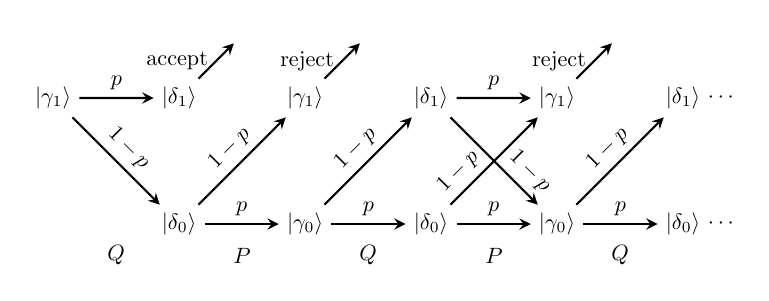
\begin{tikzpicture}[node distance=2cm, >=stealth, thick, scale=0.8, transform shape]
    \node (g-1t) at (0,2) {$|\gamma_1\rangle$};
    \node (s0t)  at (2,2) {$|\delta_1\rangle$};
    \node (s0)  at (2,0) {$|\delta_0\rangle$};
    \node (g0)  at (4,0) {$|\gamma_0\rangle$};
    \node (s1)  at (6,0) {$|\delta_0\rangle$};
    \node (g1)  at (8,0) {$|\gamma_0\rangle$};
    \node (s2)  at (10,0) {$|\delta_0\rangle$};
    \node (...1) at (10.6,0) {$\cdots$};
    \node (...2) at (10.6,2) {$\cdots$};
    
    \node (a) at (3,3) {};
    \node (r1) at (5,3) {};
    \node (r2) at (9,3) {};
    
    \node (g1t) at (4,2) {$|\gamma_1\rangle$};
    \node (s1t) at (6,2) {$|\delta_1\rangle$};
    \node (g2t) at (8,2) {$|\gamma_1\rangle$};
    \node (s2t) at (10,2) {$|\delta_1\rangle$};
    
    % Transitions
    \draw[->] (s0) -- node[above] {$p$} (g0);
    \draw[->] (g0) -- node[above] {$p$} (s1);
    \draw[->] (s1) -- node[above] {$p$} (g1);
    \draw[->] (g1) -- node[above] {$p$} (s2);
    
    \draw[->] (s0) -- node[above,sloped] {$1-p$} (g1t);
    \draw[->] (g0) -- node[above ,sloped] {$1-p$} (s1t);
    \draw[->] (s1) -- node[above left,sloped] {$1-p$} (g2t);
    \draw[->] (s1t) -- node[above] {$p$} (g2t);
    \draw[->] (g-1t) -- node[above] {$p$} (s0t);
    
    \draw[->] (s1t) -- node[above right,sloped] {$1-p$} (g1);
    \draw[->] (g1) -- node[above ,sloped] {$1-p$} (s2t);
    \draw[->] (g-1t) -- node[above ,sloped] {$1-p$} (s0);

    \draw[->] (s0t) -- node[left] {accept} (a);
    \draw[->] (g1t) -- node[left] {reject} (r1);
    \draw[->] (g2t) -- node[left] {reject} (r2);

    % Labels
    \node at (1,-0.5) {$Q$};
    \node at (3,-0.5) {$P$};
    \node at (5,-0.5) {$Q$};
    \node at (7,-0.5) {$P$};
    \node at (9,-0.5) {$Q$};
\end{tikzpicture}
    \caption{Markov chain showing the transition probability between the 4 states of a single invariant subspace $\lambda$ (with $p = p^{ae\lambda}$) upon each projective measurement. The full rejection process is a mixture of such chains weighted by $|c^{aej}_{\lambda}|^2$.}
    \label{fig:transitions}
\end{figure}
\begin{figure*}
    \begin{tikzpicture}
\begin{yquant*}
qubit {$\ket{\psi_j}$}  s;
qubit {$R:\ \ket{0}$} anc;
qubit {$F: \frac{\mathbb{I}}{2}$} f;
qubit {$M:\ \ket{0}$} m;
slash s;
slash anc;
hspace {0.1cm} -;
box {$E_a$} (s,anc,f);
["$\ket{\gamma_1}$"]
barrier (-);
box {$Q^a_0$} (s,anc,f, m);
["$\ket{\delta_0}$"]
barrier (-);
box {$P^a_0$} (s,anc,f);
["$\ket{\gamma_0}$"]
barrier (-);
box {$Q^a_1$} (s,anc,f, m);
["$\ket{\delta_1}$"]
barrier (-);
box {$P^a_0$} (s,anc,f);
["$\ket{\gamma_0}$"]
barrier (-);
box {$Q^a_1$} (s,anc,f, m);
["$\ket{\delta_1}$"]
barrier (-);
box {$P^a_1$} (s,anc,f);
["$\ket{\gamma_1}$"]
barrier (-);
\end{yquant*}
\end{tikzpicture}
\caption{A successfully completed rejection procedure. The same BSI-QPE registers $R, F$ is reused by $E_{ae}$ and every $P_s^{ae}$ and $Q_s^{ae}$; the qubit $M$ is reused by every $Q_s^{ae}$. This circuit corresponds to a term in $\mathcal{B}(2)[\rho]$ for $\{s_n\}=\{1,1\}$ and, within a single invariant subspace $\lambda$ (see Section~\ref{section:rejection}), occurs with probability $(1-p^{aej}_{\lambda})^4(p^{aej}_{\lambda})^2$. The state labels at the barriers denote the corresponding states of each invariant subspace.}
\label{fig:fullcircuit}
\end{figure*}

The iterative process proceeds as follows after measuring $s=0$ (reject) from the initial $Q_s^{ae}$ measurement: 
\begin{enumerate}
    \item Measure $P_s^{ae}$
        \begin{enumerate}
            \item If $s=1$ \textbf{terminate} as the state has returned to the approximate energy of the initial state.
            \item If $s=0$ continue.
        \end{enumerate}
    \item Measure $Q_s^{ae}$
    \item Repeat up to a maximum of $n^*$ iterations
\end{enumerate}
The two measurements $P^{ae}_s$ and $Q^{ae}_s$ do not scatter the state over the whole Hilbert space. They confine it to a family of mutually orthogonal \emph{two-dimensional} subspaces, and within any one of them the state simply ping-pongs between two pairs of vectors, $\ket{\gamma_0},\ket{\gamma_1}$ and $\ket{\delta_0},\ket{\delta_1}$, according to the four-state Markov chain of Fig.~\ref{fig:transitions}. Reaching $\ket{\gamma_1}$ means the rewind has succeeded and the state has returned to its original energy. Because the chain is this simple, the probability that $n^*$ attempts all fail can be read off directly, which is what Eq.~\eqref{eq:probabilty_of_rejection} does. 

To see this let us consider the action of the rejection process on each eigenvector $\ket{\psi_j}$ of $H$. To handle the mixed initial state of $F$, purify $\frac{\mathbb{I}}{2}$ as $\ket{\Phi}_{FF'}=\frac{1}{\sqrt{2}}\sum_f\ket{f}_F\ket{f}_{F'}$, where the reference $F'$ is never acted upon. Conditioned on the outcome $(a,e)$, the corresponding pure post-measurement state is
\begin{equation}
    \frac{(E_{ae}\otimes\mathbb I_{F'})\ket{\psi_j}\ket{0}_R\ket{\Phi}_{FF'}\ket{0}_M}
    {\|(E_{ae}\otimes\mathbb I_{F'})\ket{\psi_j}\ket{0}_R\ket{\Phi}_{FF'}\ket{0}_M\|}
    = \sum_{\lambda} c_{\lambda}^{aej}\ket{\gamma_1^{ae \lambda}}.
\end{equation}
Tracing out $F'$ recovers the physical evolution from $\frac{\mathbb{I}}{2}$. Because $P_1^{ae}E_{ae}=E_{ae}$, this state is a $+1$ eigenstate of $P_1^{ae}$ (with all projectors implicitly extended by $\mathbb I_{F'}$). Furthermore, $P_1^{ae}$ commutes with $P^{ae}_1Q^{ae}_0P^{ae}_1$, so the two operators are jointly diagonalizable and the expansion above may be taken in their joint eigenstates. The untouched reference is absorbed into the degeneracy label $\lambda$.
Writing the eigenvalue of $\ket{\gamma^{ae\lambda}_1}$ as $1-p^{ae\lambda}$, we have: \begin{align}1-p^{ae\lambda}&=\bra{\gamma^{ae\lambda}_1}P^{ae}_1Q^{ae}_0P^{ae}_1\ket{\gamma^{ae\lambda}_1} \\&=\|Q^{ae}_0P^{ae}_1\ket{\gamma^{ae\lambda}_1}\|^2\\ &= 1-\|Q^{ae}_1\ket{\gamma^{ae\lambda}_1}\|^2
\end{align}
so $p^{ae\lambda} = \|Q^{ae}_1\ket{\gamma^{ae\lambda}_1}\|^2$, and the probability of accepting the update is given by the mixture $p_{aej} = \sum_{\lambda}|c^{aej}_{\lambda}|^2p^{ae\lambda}$. Therefore, for each $\lambda$ with $p^{ae\lambda} \in (0,1)$ we can define the following 2D invariant subspace (we have suppressed the $ae\lambda$ labels for the remainder of this section for clarity, writing $\ket{\gamma_1} = \ket{\gamma^{ae\lambda}_1}$ and $p = p^{ae\lambda}$):
\begin{align}
    \ket{\delta_0} &= \frac{Q^{ae}_0P^{ae}_1\ket{\gamma_1}}{\sqrt{1-p}} &\ket{\delta_1} &= \frac{Q^{ae}_1P^{ae}_1\ket{\gamma_1}}{\sqrt{p}} \\
    \ket{\gamma_0} &= \frac{P^{ae}_0Q^{ae}_0\ket{\delta_0}}{\sqrt{p}} &\ket{\gamma_1} &= \frac{P^{ae}_1Q^{ae}_0\ket{\delta_0}}{\sqrt{1-p}}
\end{align}
From these definitions the following relations can be deduced:
\begin{align}
\begin{split}
\label{eq:deltagamma0}
    P^{ae}_1 \ket{\gamma_1} &= (Q^{ae}_0+Q^{ae}_1)P^{ae}_1 \ket{\gamma_1}\\
    &= Q^{ae}_0P^{ae}_1 \ket{\gamma_1}+Q^{ae}_1P^{ae}_1 \ket{\gamma_1}\\
    &= \sqrt{1-p} \ket{\delta_0} + \sqrt{p}\ket{\delta_1}\\
    Q^{ae}_0\ket{\delta_0} &= \sqrt{p} \ket{\gamma_0} + \sqrt{1-p} \ket{\gamma_1}
\end{split}
\end{align}
As $P^{ae}_1 \ket{\gamma_1} = \ket{\gamma_1}$ and $Q^{ae}_0\ket{\delta_0} = \ket{\delta_0}$ we can simplify the above and then through substitution deduce the remaining relations:
\begin{align}
\begin{split}
\label{eq:deltagamma1}
        \ket{\delta_1} &= -\sqrt{1-p} \ket{\gamma_0} + \sqrt{p} \ket{\gamma_1}\\
    \ket{\gamma_0} &= \sqrt{p} \ket{\delta_0} - \sqrt{1-p}\ket{\delta_1}
\end{split}
\end{align}
Therefore it is clear that each measurement transitions the state from one of $\ket{\delta_i}$ to one of $\ket{\gamma_i}$ or vice versa, whilst remaining within the same 2D invariant subspace. As the subspaces corresponding to different $\lambda$ are mutually orthogonal (which follows from the orthogonality of the $\ket{\gamma^{ae\lambda}_1}$ together with the relations above) and each is preserved by both measurements, the subspaces do not mix at any point during the rejection process. The probability of these transitions are trivially deduced from \eqref{eq:deltagamma0} and \eqref{eq:deltagamma1}, and can be seen in Fig.~\ref{fig:transitions}.


From this we can calculate the probability of attempting to reject and then failing the rejection process within a single invariant subspace to be $p(1-p)(p^2 +(1-p)^2)^{n^*}$. As the subspaces do not mix, the overall failure probability $p_a^{fail}$ is the corresponding mixture over subspaces (reinstating the suppressed labels):
\begin{equation}
   p_{aej}^{fail} =  \sum_{\lambda}|c^{aej}_{\lambda}|^2p^{ae\lambda}(1-p^{ae\lambda})((p^{ae\lambda})^2 +(1-p^{ae\lambda})^2)^{n^*}
\end{equation}
For all $p \in [0,1]$ we have: 
\begin{equation}
    p(1-p)(p^2 +(1-p)^2)^{n^*} \leq \frac{1}{2(n^*+1)} \left(\frac{n^*}{n^*+1}\right)^{n^*}
\end{equation}
Therefore, as $\sum_{\lambda}|c^{aej}_{\lambda}|^2=1$ we have:
\begin{equation}
    \label{eq:probabilty_of_rejection}
   p_{aej}^{fail} \leq \frac{1}{2(n^*+1)} \left(\frac{n^*}{n^*+1}\right)^{n^*} \leq \frac{1}{2n^*}
\end{equation}
If the rejection process fails then the whole algorithm fails irrecoverably and must be reset to the original initial state.

We have chosen to present the rewinding mechanism through this lens of projective measurements and invariant subspaces in an attempt to make the procedure more intuitive. We refer the reader to the treatment via Jordan's Lemma in the original Quantum Metropolis paper \cite{Temme_2011} for an alternative approach to reach the same conclusions.
\label{section:rejection}

\section{Why it works}
\label{section:why}
The classical Metropolis-Hastings algorithm works by constructing a Markov Chain through proposing and accepting/rejecting moves with probabilities determined by the energy difference between the initial and modified states. The transition matrix of this Markov chain is in detailed balance with respect to the Gibbs state, implying that the Gibbs state is a fixed point of the Markov chain. As Markov chain is also ergodic, it is known that it must have a single unique fixed point and converge towards it. Therefore, the Markov chain converges to the Gibbs state.

In the quantum Metropolis algorithm we similarly construct a quantum Markov chain by proposing and accepting or rejecting moves based on energy differences. Because the energy differences cannot be resolved exactly, we cannot prove exact detailed balance and instead use a notion of approximate quantum detailed balance (Definition~\ref{def:approxdb}) that incorporates additive errors from the nonzero, exponentially suppressed tails of BSI-QPE. We use this theorem to establish that the Gibbs state is approximately invariant. Further choosing the update set $\{C\}$ to be universal ensures ergodicity and hence the uniqueness of the fixed point \cite{Temme_2011}. The closeness of the actual fixed point to this approximately invariant point additionally depends on the mixing properties of the channel. We formalise these statements into the following main result of the paper. Informally, it says: \emph{one round of the algorithm moves the Gibbs state only a little, and the two ways it can move are both controllable --- by adding ancilla qubits, and by allowing more rewinding attempts.} Formally:

\begin{theorem}
\label{theorem:main}
Let $\mathcal{E}$ be one update round of the quantum Metropolis algorithm of Section~\ref{section:algorithm}, implemented with $\eta$ ancillas, evolution time $t = \frac{1}{16\|H\|}$, rewinding cap $n^*$, an update measure satisfying $d\mu(C)=d\mu(C^{\dagger})$, and window functions satisfying the conditions of Appendix~\ref{section:appendix} with truncation bandwidth $\mu = \Omega(\frac{1}{\nu}\log n^*)$, $\mu < \min(\frac{N}{96\pi}, \frac{\frac{N}{8}}{4n^*+6}, \frac{Nt}{384\pi\beta(4n^*+6)})$. Then
\begin{equation}
   \|\mathcal{E}[\sigma_G] - \sigma_G\|_* = O\left(\max\left( n^{*\frac{7}{2}}\sqrt{\frac{\beta\|H\| }{2^{\eta}}}\mu^{\frac{3}{2}},\frac{1}{n^*}\right)\right).
\label{eq:theoremmain}
\end{equation}
If, in addition, $\mathcal{E}^{\ell}$ is strictly trace-norm contracting with factor $k<1$ for some integer $\ell\geq1$, then $\mathcal{E}$ has a unique fixed point $\sigma^*$, is approached exponentially fast, and $\|\sigma^*-\sigma_G\|_* \leq \frac{\ell}{1-k}\|\mathcal{E}[\sigma_G] - \sigma_G\|_*$ (Theorem~\ref{theorem:error_bound}). If moreover $\frac{\ell}{1-k}\leq\tau_0$ with $\tau_0$ independent of $\eta$, $n^*$ and the window parameters, then $\sigma_G$ is prepared to any trace-norm accuracy at polynomial cost (Corollary~\ref{corollary:polycost}).
\end{theorem}

The two terms in Eq.~\eqref{eq:theoremmain} have quite different origins, and it is worth separating them before the proof. The first, $n^{*\frac{7}{2}}\sqrt{\beta\|H\|2^{-\eta}}\mu^{\frac{3}{2}}$, is the residual \emph{bias} left by an imperfect energy estimate: the acceptance probability is computed from a readout that is only accurate to within the bandwidth $\mu$, so detailed balance holds only up to a multiplicative error, and every extra rewinding attempt gives that error another chance to act. It shrinks exponentially in the number of ancilla qubits $\eta$. The second, $1/n^*$, is the probability that the rewind never terminates and the whole run must be discarded (Eq.~\eqref{eq:probabilty_of_rejection}); it shrinks as the cap $n^*$ is raised.

The proof of this theorem occupies the remainder of this section and is broken down into a number of steps. First, in Section~\ref{section:detailedbalancedef} we define our approximate detailed balance criteria which allow us to consider each branch of the original $\mathcal{E}$ CP-map separately. We then proceed in Section~\ref{section:proofbranchwisebalance} to prove the acceptance and rejection branches of our update step satisfy our branch-wise approximate detailed balance criteria. Finally, in Section~\ref{sec:combine} use Lemma~\ref{theorem:quantumapproximatedeatildedbalance} to combine these error terms to demonstrate that the Gibbs state is approximately stationary. We go further and show that by taking certain assumptions we can show the Gibbs state is close to the fixed point of the map, and that the map converges exponentially quickly towards this fixed point.
\section{Approximate Quantum Detailed Balance}
\label{section:detailedbalancedef}
In the classical setting, detailed balance can be verified by comparing each transition with its reverse, weighted by the Gibbs probabilities. Our attempts to replicate this methodology in the quantum setting are frustrated by two obstacles. First, due to inexact quantum phase estimation, we cannot exactly resolve the energies of our states and hence cannot implement the exact transition amplitudes that would lead to quantum detailed balance. Second, some branches of the weighted adjoint map agree closely not with the corresponding branch of the original map, but with a differently labelled one. In this section we therefore present a formulation of approximate quantum detailed balance that is verified branch by branch, allows branches to be paired with differently labelled partners, and accommodates the additive errors introduced by the truncation step.

For any completely positive map $\mathcal{M}$ with Kraus decomposition $\mathcal{M}[\rho] = \sum_{j} A_{j}\rho A^{\dagger}_{j}$ and any density matrix $\sigma$, we define
\begin{align}
    \mathcal{M}_{\sigma}[\rho] &= \sum_{j} A_{j}\sigma^{\frac{1}{2}}\rho\,\sigma^{\frac{1}{2}} A^{\dagger}_{j} = \mathcal{M}\big[\sigma^{\frac{1}{2}}\rho\,\sigma^{\frac{1}{2}}\big],\\
    \mathcal{M}^{\dagger}[\rho] &= \sum_j A^{\dagger}_j \rho A_j,\\
    \mathcal{M}^*_{\sigma}[\rho] &= \sum_{j} \sigma^{\frac{1}{2}}A^{\dagger}_{j}\rho A_{j}\sigma^{\frac{1}{2}} = \sigma^{\frac{1}{2}}\mathcal{M}^{\dagger}[\rho]\,\sigma^{\frac{1}{2}}.
\end{align}

\begin{definition}[Approximate quantum detailed balance]
\label{def:approxdb}
A completely positive map $\mathcal{M}$ satisfies $\epsilon$-approximate quantum
detailed balance with respect to $\sigma$ if, for every operator $X$,
\begin{equation}
    \|\mathcal{M}^*_{\sigma}[X] - \mathcal{M}_{\sigma}[X]\|_* \leq \epsilon\|X\|.
\end{equation}
\end{definition}

Our strategy is to establish the $X=\mathbb{I}$ instance of Definition~\ref{def:approxdb}, which is all Lemma~\ref{theorem:quantumapproximatedeatildedbalance} requires, for each acceptance and rejection branch of $\mathcal{E}$ separately. Lemma~\ref{lemma:1} compares components paired by a relabelling $c\mapsto c'$. For each input basis state, its hypothesis requires the corresponding weighted outputs to differ only by a small diagonal rescaling; its conclusion converts these multiplicative discrepancies $\epsilon_{m}$ into a trace-norm bound. The lemma is stated for two maps $\mathcal{M}$ and $\mathcal{M}'$ because, in the rejection step, we can establish this criterion only after slightly modifying the acceptance rotations in the weighted adjoint map. We bound the error introduced by this modification separately.

\begin{lemma}[Branch-wise Approximate Detailed Balance Criterion]
\label{lemma:1}
Let $\mathcal{M}$ and $\mathcal{M'}$ be completely positive maps on $d$-dimensional density matrices admitting the same decomposition $\mathcal{M} = \sum_{c\in\mathcal{X}} \mathcal{M}_c$, $\mathcal{M'} = \sum_{c\in\mathcal{X}} \mathcal{M'}_c$ into completely positive maps $\mathcal{M}_c$ and $\mathcal{M}'_c$, and let $\sigma = \sum_j \sigma_j \ket{\psi_j}\bra{\psi_j}$ be a density matrix diagonal in the orthonormal basis $\{\ket{\psi_j}\}$. Suppose there exists a bijection $c \mapsto c'$ of $\mathcal{X}$ such that, for every $j,k,c,l,m$,
\begin{equation}
    \bra{\psi_m}\mathcal{M}^{\prime *}_{c'\sigma}[\ket{\psi_j}\bra{\psi_k}]\ket{\psi_l}
    =(1+u^{c}_{jm})(1+ u^{c}_{kl})
    \bra{\psi_m}\mathcal{M}_{c\sigma}[\ket{\psi_j}\bra{\psi_k}]\ket{\psi_l}
    \label{eq:approximate_quantum_detailed_balance_condition}
\end{equation}
where the $u^{c}_{jl}$ are real and satisfy $|u^{c}_{jl}| \leq \epsilon_m$. Then, for every operator $X$,
 \begin{equation}
    \|\mathcal{M}^{\prime *}_{\sigma}[X]-\mathcal{M}_{\sigma}[X] \|_* \leq (2\epsilon_m+\epsilon_m^2)\|\mathcal{M}[\sigma]\|_*\|X\| \label{eq:lemma2output}
\end{equation}
where $\|\cdot\|_*$ is trace-norm.
\end{lemma}

\begin{proof}
 By definition $\mathcal{M}[\sigma]=\mathcal{M}_{\sigma}[\mathbb{I}]$. By linearity and the bijectivity of $c \mapsto c'$:
    \begin{equation}
        \mathcal{M}^{\prime *}_{\sigma}[X] = \sum_{c}\mathcal{M}^{\prime *}_{c\sigma}[X] = \sum_{c}\mathcal{M}^{\prime *}_{c'\sigma}[X]
    \end{equation}
    Define $M^{jc} = \mathcal{M}_{c\sigma}[\ket{\psi_j}\bra{\psi_j}]$ and $D^{jc}=\sum_l(1+u_{jl}^{c})\ket{\psi_l}\bra{\psi_l}$, let $\mathcal{M}_{c\sigma}[\rho]=\sum_i K^c_i\rho K^{c\dagger}_i$ be a Kraus decomposition, and let $\tilde K^c_i=\sum_j D^{jc}K^c_i\ket{\psi_j}\bra{\psi_j}$. Equation~\eqref{eq:approximate_quantum_detailed_balance_condition} is then, by linearity, the operator identity
    \begin{equation}
        \mathcal{M}^{\prime *}_{c'\sigma}[X]=\sum_i\tilde K^c_iX\tilde K^{c\dagger}_i
    \end{equation}
    Moreover, $\mathcal{M}_{\sigma}[X] = \sum_{i,c}K^c_iXK^{c\dagger}_i$, so we have:
    \begin{equation}
        \|\mathcal{M}^{\prime *}_{\sigma}[X]-\mathcal{M}_\sigma[X]\|_* \leq \sum_{i,c}\Big\|\left(\tilde K^c_iX\tilde K^{c\dagger}_i-K^c_iXK^{c\dagger}_i\right)\Big\|_*
    \end{equation}
    Writing $W^c_i=\tilde K^c_i-K^c_i$, we have:
    \begin{equation}
        \tilde K^c_iX\tilde K^{c\dagger}_i-K^c_iXK^{c\dagger}_i = W^c_iXK^{c\dagger}_i + K^c_iXW^{c\dagger}_i + W^c_iXW^{c\dagger}_i
    \end{equation}
    By the generalised H\"older's inequality for Schatten norms we have:
    \begin{equation}
        \Big\|W^c_iXK^{c\dagger}_i\Big\|_* \leq \|W^c_i\|_2\|X\| \|K^{c\dagger}_i\|_2
    \end{equation}
    Further by Cauchy-Schwarz:
    \begin{equation}
        \sum_i\Big\|W^c_iXK^{c\dagger}_i\Big\|_* \leq \|X\| \sqrt{\sum_i \|W^c_i \|^2_2}\sqrt{\sum_i \|K_i^{c\dagger}\|^2_2}
    \end{equation}
    and similarly for the remaining terms. We have 
    
    \begin{align}
        \sum_i \|K^{c\dagger}_i\|^2_2&=\sum_i\operatorname{Tr}[K^{c\dagger}_iK^{c}_i]=\operatorname{Tr}[\mathcal{M}_{c\sigma}[\mathbb{I}]]\\
        &=\sum_j \operatorname{Tr}[M^{jc}]
    \end{align} and similarly $\sum_i \|W^c_i\|^2_2=\sum_j \operatorname{Tr}[V^{jc}M^{jc}V^{jc}]$ where $V^{jc} = D^{jc}-\mathbb{I}$, which satisfies $\|V^{jc}\|\leq\epsilon_m$. Further, as $M^{jc}$ is positive semi-definite:
    \begin{equation}
       \operatorname{Tr}[V^{jc}M^{jc}V^{jc}] \leq \|V^{jc}\|^2\, \operatorname{Tr}[M^{jc}] \leq \epsilon_m^2\, \operatorname{Tr}[M^{jc}]
    \end{equation}
    Therefore,
    \begin{equation}
        \|\mathcal{M}^{\prime *}_{\sigma}[X]-\mathcal{M}_\sigma[X]\|_* 
        \leq (2\epsilon_m+\epsilon_m^2)\|X\|\sum_{j,c}\operatorname{Tr}[M^{jc}] 
    \end{equation}
    Finally:
    \begin{equation}
        \sum_{j,c}\operatorname{Tr}[M^{jc}] = \operatorname{Tr}[\mathcal{M}_{\sigma}[\mathbb{I}]] = \operatorname{Tr}[\mathcal{M}[\sigma]] = \|\mathcal{M}[\sigma]\|_*
    \end{equation}
\end{proof}

We use Lemma~\ref{lemma:1} to show that our band-limited maps satisfy the branch-wise approximate detailed balance
criterion for the acceptance branch $\tilde{\mathcal{A}}$ and every rejection branch $\tilde{B}(n)$. We then add the additive error ($\epsilon_a$) between the original map and the band-limited map to show approximate quantum detailed balance for the acceptance and rejection branches. Finally, we combine these using Lemma~\ref{theorem:quantumapproximatedeatildedbalance} to show the Gibbs state is approximately stationary.
\begin{lemma}[Approximate detailed balance implies approximate stationarity]
\label{theorem:quantumapproximatedeatildedbalance}
Let $\mathcal{E} = \sum_j \mathcal{M}_j$ be a completely positive trace-preserving map on $d$-dimensional density matrices, with each $\mathcal{M}_j$ completely positive, and let $\sigma$ be a density matrix. If each $\mathcal{M}_j$ satisfies $\epsilon^j$-approximate quantum detailed balance with respect to $\sigma$ (Definition~\ref{def:approxdb}), or merely its $X=\mathbb{I}$ instance, then
\begin{equation}
     \|\mathcal{E}[\sigma]-\sigma\|_* \leq \sum_j\min\left(\epsilon^j, 2\|\mathcal{M}_j[\sigma]\|_*\right)
\end{equation}
\end{lemma}
\begin{proof}
    By the triangle inequality we have:
    \begin{equation}
        \|\mathcal{E}^*_{\sigma}[\mathbb{I}]-\mathcal{E}[\sigma]\|_* \leq \sum_j \|\mathcal{M}^*_{j\sigma}[\mathbb{I}]-\mathcal{M}_{j}[\sigma]\|_*
    \end{equation}
    As $\mathcal{E}$ is trace-preserving, we know that:
    \begin{equation}
        \mathcal{E}^*_{\sigma}[\mathbb{I}] = \sum_{j} \sigma^{\frac{1}{2}}A^{\dagger}_{j} A_{j}\sigma^{\frac{1}{2}} = \sigma
    \end{equation}
    Therefore,
    \begin{equation}
        \|\sigma - \mathcal{E}[\sigma]\|_* \leq \sum_j \|\mathcal{M}^*_{j\sigma}[\mathbb{I}]-\mathcal{M}_{j}[\sigma]\|_*
    \end{equation}
    By assumption (with $X=\mathbb{I}$, $\|\mathbb{I}\|=1$) we have
    \begin{equation}
        \|\mathcal{M}^*_{j\sigma}[\mathbb{I}]-\mathcal{M}_{j}[\sigma]\|_* \leq \epsilon^j
    \end{equation}
    Further, as both
$\mathcal{M}_{j,\sigma}^{*}[\mathbb{I}]$ and
$\mathcal{M}_j[\sigma]$ are positive semidefinite:
    \begin{align}
        \|\mathcal{M}^*_{j\sigma}[\mathbb{I}]\|_* &= Tr\left[\sum_l \sigma^{\frac{1}{2}} K_{jl}^{\dagger} \mathbb{I} K_{jl} \sigma^{\frac{1}{2}}\right]\\
        &= Tr\left[\sum_l K_{jl}\sigma K_{jl}^{\dagger}\right]\\
        &= \|\mathcal{M}_{j}[\sigma]\|_*
    \end{align}
    Therefore,
    \begin{equation}
         \|\mathcal{M}^*_{j\sigma}[\mathbb{I}]-\mathcal{M}_{j}[\sigma]\|_* \leq 2\|\mathcal{M}_{j}[\sigma]\|_*
    \end{equation}
    Hence,
    \begin{equation}
        \|\sigma-\mathcal{E}[\sigma]\|_* \leq \sum_j \min \left(\epsilon^j, 2\|\mathcal{M}_{j}[\sigma]\|_*\right)
    \end{equation}
\end{proof}

% \begin{widetext}
\subsection{Proof of Theorem~\ref{theorem:main}}
\label{section:proofmain}
We must first express $\mathcal{E}$ as a completely positive trace preserving map:
\begin{equation}
    \mathcal{E}[\rho] = \mathcal{A}[\rho] + \sum_{n=0}^{n^*} \mathcal{B}(n)[\rho] + \mathcal{C}[\rho]
\end{equation}
where $\mathcal{A}$ corresponds to acceptance, $\mathcal{B}(n)$ to successful rejection after $n$ iterations and $\mathcal{C}$ to failing to reject after $n^*$ iterations. Let $\Omega_{RFM} =\ket{0}\bra{0}_R\otimes \frac{\mathbb{I}_F}{2}\otimes\ket{0}\bra{0}_M$ denote the initial state of the persistent ancillas. All occurrences of $E_{ae}$, $P_s^{ae}$, $Q_s^{ae}$ and $L_b^{ade}$ below act on this common ancillary space, with identities on any register on which a given operator acts trivially. Then
\begin{equation}
    \mathcal{A}[\rho] = \int  Tr_{RFM}\bigg[\sum_{a,b,d,e}L_b^{ade} E_{ae} ( \rho\otimes \Omega_{RFM}) 
     E_{ae}L^{ade\dagger}_b\bigg]d\mu(C)
\end{equation}
\begin{equation}
    \mathcal{B}(n)[\rho] = \int Tr_{RFM}\bigg[\sum_{a,e,\{s\}}P^{ae}_1Q^{ae}_{s_n}\ldots P^{ae}_0Q^{ae}_{s_1}P^{ae}_0Q^{ae}_0E_{ae} ( \rho\otimes \Omega_{RFM})E_{ae}Q^{ae}_0P^{ae}_0Q^{ae}_{s_1}P^{ae}_0\ldots Q^{ae}_{s_n}P^{ae}_1\bigg]d\mu(C)
\end{equation}
\begin{equation}
    \mathcal{C}[\rho] = \rho_0 \int Tr\bigg[\sum_{a,e,\{s\}}P^{ae}_0Q^{ae}_{s_{n^*}}\ldots P^{ae}_0Q^{ae}_{s_1}P^{ae}_0Q^{ae}_0E_{ae} ( \rho\otimes \Omega_{RFM})E_{ae}Q^{ae}_0P^{ae}_0Q^{ae}_{s_1}P^{ae}_0\ldots Q^{ae}_{s_{n^*}}P^{ae}_0\bigg]d\mu(C) 
\end{equation}
where $\rho_0$ is the initial state the overall Metropolis algorithm was started from. 
\paragraph{Approximate quantum detailed balance of $\mathcal{A}$ and $\mathcal{B}$}
\label{section:proofbranchwisebalance}
We demonstrate that $\mathcal{A}$ and $\mathcal{B}$ are in approximate detailed balance by proving \eqref{eq:approximate_quantum_detailed_balance_condition} holds for each of them. We achieve this via the same 4 step proof applied to each map. Here we give a high-level overview of the proof steps, with the proofs themselves laid out in Appendices~\ref{appendix:Aproof} and \ref{appendix:Bproof}:
\begin{enumerate}
    \item \textbf{Truncate.} We replace $\hat \alpha$, $\hat \beta$ by their band-limited versions $\tilde \alpha$, $\tilde \beta$ as in Lemma~\ref{lemma:0}. Then, we use Lemma~\ref{lemma:3} to bound the diamond-norm difference between the original $E^{ae}$, $P_s^{ae}$, $Q_s^{ae}$ measurements and their band-limited replacements. Using Lemma~\ref{lemma:composition} we combine these bounds on the error of each measurement into a diamond-norm bound on the difference between the band-limited map ($\tilde{\mathcal{A}}$, $\tilde{\mathcal{B}}$) and the original ($\mathcal{A}$, $\mathcal{B}$):
        \begin{equation}
    \begin{aligned}
    \|\mathcal{A}_{\sigma_G}[\mathbb{I}] - \tilde{\mathcal{A}}_{\sigma_G}[\mathbb{I}]\|_*  &\leq 24e\epsilon_{\Delta}\\
    \|\mathcal{A}^*_{\sigma_G}[\mathbb{I}] - \tilde{\mathcal{A}}^*_{\sigma_G}[\mathbb{I}]\|_* &\leq 24e\epsilon_{\Delta}
    \end{aligned}
    \label{eq:suma1}
\end{equation}
    \begin{equation}
    \begin{aligned}
    \|\mathcal{B}_{\sigma_G}(n)[\mathbb{I}] - \tilde{\mathcal{B}}_{\sigma_G}(n)[\mathbb{I}]\|_* &\leq 24e(2n+3)\epsilon_{\Delta}
    \\ \|\mathcal{B}^*_{\sigma_G}(n)[\mathbb{I}] - \tilde{\mathcal{B}}^*_{\sigma_G}(n)[\mathbb{I}]\|_* &\leq 24e(2n+3)\epsilon_{\Delta}
    \end{aligned}
    \label{eq:sumb1}
\end{equation}
    \item \textbf{Reverse Histories.} By relabeling the indices corresponding to the measurement outcomes we are able to (approximately) relate a branch of the adjoint map with one of the original map up to the Boltzmann factors. A branch of the adjoint map describes the round run backwards, and the relabelling is nothing more than reading the measurement record from the end to the beginning. In the acceptance branch this requires that the move distribution weights $C$ and $C^{\dagger}$ equally ($d\mu(C) = d\mu(C^{\dagger})$). For the rejection branch we do not relate the branches of the adjoint map directly to those of the original ($\mathcal{B}$) but instead relate them to a slightly perturbed approximation ($\mathcal{T}$) of the original map.
    
    \item \textbf{Support.} Band-limiting means that only a narrow set of measurement outcomes contribute. By considering the restricted support of the band-limited operations we are able to find the subset of possible measurement outcomes when acting upon a given input state.
    \item \textbf{Reweight}. Using the restricted support of the band-limited BSI-QPE we finish relating the adjoint map with the original map by exchanging the Boltzmann factors up to a multiplicative error:
    \begin{multline}
  \bra{\psi_m}\tilde{\mathcal{A}}^*_{b+N-z,a+N-z,e,d,N-z,\sigma_G}[\ket{\psi_j}\bra{\psi_k}]\ket{\psi_l} 
   =\\(1+u_{jm}^{abdez})(1+u_{kl}^{abdez})\bra{\psi_m}\tilde{\mathcal{A}}_{abdez,\sigma_G}[\ket{\psi_j}\bra{\psi_k}]\ket{\psi_l}
   \label{eq:Aconditioneq}
\end{multline}
\begin{equation}
    \bra{\psi_m}\tilde{\mathcal{T}}^*_{N -z,\sigma_G}(n)[\ket{\psi_j}\bra{\psi_k}]\ket{\psi_l}
    =(1+v_{kl})(1+v_{jm})\bra{\psi_m}\tilde{\mathcal{B}}_{z,\sigma_G}(n)[\ket{\psi_j}\bra{\psi_k}]\ket{\psi_l}
    \label{eq:Bconditioneq}
\end{equation}
    where $|u_{jr}^{abde}| \leq \epsilon_{\mathcal{A}} = O(\frac{\beta \mu}{Nt})$ and $|v_{jr}| \leq \epsilon_{\mathcal{B}} = O(\frac{n\beta \mu}{Nt})$. For the rejection branch we additionally must demonstrate the perturbed map we introduced in \textbf{Reverse Histories} is indeed close to the original map:
\begin{equation}
    \|\tilde{\mathcal{T}}(n) - \tilde{\mathcal{B}}(n)\|_{\diamond} \leq 36e(n+1)\sqrt{\beta\frac{6\pi}{Nt}}((4n+6)\mu)^{\frac{3}{2}}+72e(n+1)(4n+6)\mu\epsilon_{\Delta}
    \label{eq:Wdrifterrormain}
\end{equation}
\end{enumerate}
By applying Lemma~\ref{lemma:1} to \eqref{eq:Aconditioneq} and \eqref{eq:Bconditioneq} we are able to see that:
\begin{equation}
    \|\tilde{\mathcal{A}}^*_{\sigma_G}[\mathbb{I}] - \tilde{\mathcal{A}}_{\sigma_G}[\mathbb{I}]\|_* \leq (2\epsilon_{\mathcal{A}}+ \epsilon_{\mathcal{A}}^2)\|\tilde{\mathcal{A}}_{\sigma_G}[\mathbb{I}]\|_*
    \label{eq:Aoutput}
\end{equation}
\begin{equation}
    \|\tilde{\mathcal{T}}^*_{\sigma_G}(n)[\mathbb{I}] - \tilde{\mathcal{B}}_{\sigma_G}(n)[\mathbb{I}]\|_* \leq (2\epsilon_{\mathcal{B}} + \epsilon_{\mathcal{B}}^2)\|\tilde{\mathcal{B}}_{\sigma_G}(n)[\mathbb{I}]\|_*
    \label{eq:Boutput}
\end{equation}
Hence, combining these with \eqref{eq:suma1}, \eqref{eq:sumb1} and \eqref{eq:Wdrifterrormain} we get:
\begin{equation}
    \|\mathcal{A}^*_{\sigma_G}[\mathbb{I}] - \mathcal{A}_{\sigma_G}[\mathbb{I}]\|_* = O\!\left(\frac{\beta\mu}{Nt}\right)\|\mathcal{A}_{\sigma_G}[\mathbb{I}]\|_* + O\!\left(\epsilon_{\Delta}\right)
\end{equation}
\begin{multline}
    \|\mathcal{B}^*_{\sigma_G}(n)[\mathbb{I}] - \mathcal{B}_{\sigma_G}(n)[\mathbb{I}]\|_* = O\left(\frac{(n+2)\beta\mu}{Nt} \right)\|\mathcal{B}_{\sigma_G}(n)[\mathbb{I}]\|_* +\\O\left(\max\left((n+2)^2\mu\epsilon_{\Delta},(n+2)^{\frac{5}{2}}\sqrt{\frac{\beta }{Nt}}\mu^{\frac{3}{2}}\right)\right) 
\end{multline}
Thus, we demonstrate the $X=\mathbb{I}$ instance of approximate quantum detailed balance for $\mathcal{A}$ and $\mathcal{B}$, which suffices for Lemma~\ref{theorem:quantumapproximatedeatildedbalance}.
\paragraph{Combining error contributions}
\label{sec:combine}
Using Lemma~\ref{theorem:quantumapproximatedeatildedbalance} we can combine these results, taking for each map the $\epsilon^j$ established above. Table~\ref{tab:contributions} highlights the origin of all the error terms.
\begin{table}[htbp]
\centering
\setlength{\tabcolsep}{6pt}
\renewcommand{\arraystretch}{1.3}
\begin{tabular}{@{}lll@{}}
\toprule
Contribution & Bound & Established in \\
\midrule
$\mathcal{A}$: truncation & $O(\epsilon_{\Delta})$ & Eq.~\eqref{eq:AAtildeclose2} \\
$\mathcal{A}$: reweighting & $O(\beta\mu/Nt)\,\|\mathcal{A}[\sigma_G]\|_*$ & Eq.~\eqref{eq:Aoutput} \\
$\mathcal{B}(n)$: truncation & $O((2n+3)\epsilon_{\Delta})$ & Eq.~\eqref{eq:Bsrelation} \\
$\mathcal{B}(n)$: reweighting & $O((n+2)\beta\mu/Nt)\,\|\mathcal{B}(n)[\sigma_G]\|_*$ & Eq.~\eqref{eq:Boutput} \\
$\mathcal{B}(n)$: $W$-drift & $O\big(\max\big((n+2)^2\mu\epsilon_{\Delta},\,(n+2)^{5/2}\sqrt{\beta/Nt}\,\mu^{3/2}\big)\big)$ & Eq.~\eqref{eq:Wdrifterror} \\
$\mathcal{C}$: failure mass & $2\|\mathcal{C}[\sigma_G]\|_* \leq 1/n^*$ & Eq.~\eqref{eq:probabilty_of_rejection} \\
\bottomrule
\end{tabular}
\caption{\label{tab:contributions} Origins of error terms contributing to Eq.~\eqref{eq:combinedtotalerror}.}
\end{table}


From $\mathcal{A}$, as $\|\mathcal{A}[\sigma_G]\|_* \leq 1$, the contribution to the total error is given by $O(\max(\frac{8\pi}{Nt}\beta\mu,\epsilon_{\Delta}))$. From $\sum_n\mathcal{B}(n)$ the contribution to the total error is given by:
\begin{equation}
    O\!\bigg(\max\!\bigg(\sum_{n=0}^{n^*}\|\mathcal B(n)[\sigma_G]\|_* (n+2)\frac{8\pi}{Nt}\beta \mu,
    \sum_{n=0}^{n^*}(n+2)^2\mu\epsilon_{\Delta}, \sum_{n=0}^{n^*}(n+2)^{\frac{5}{2}}\sqrt{\frac{\beta }{Nt}}\mu^{\frac{3}{2}}\bigg)\bigg)
\end{equation}
By following a similar logic to the derivation of Eq.~\eqref{eq:probabilty_of_rejection}, we have $\|\mathcal B(n)[\sigma_G]\|_* = O(n^{-2})$ for $n\geq1$. Therefore, the total contribution from $\mathcal{B}$ is $O(\!\max(\frac{8\pi}{Nt}\beta \mu \log n^*,n^{*3}\mu\epsilon_{\Delta},n^{*\frac{7}{2}}\sqrt{\frac{\beta }{Nt}}\mu^{\frac{3}{2}}))$. From $\mathcal{C}$ the contribution is simply $2\|\mathcal{C}[\sigma_G]\|_* = O(\frac{1}{n^*})$. Therefore,
 \begin{equation}
   \epsilon_c = \|\mathcal{E}[\sigma_G] - \sigma_G\|_* = O\bigg(\max\bigg( \frac{8\pi}{Nt}\beta\mu \log n^* ,\frac{1}{n^*}, n^{*3}\mu\epsilon_{\Delta},n^{*\frac{7}{2}}\sqrt{\frac{\beta }{Nt}}\mu^{\frac{3}{2}}\bigg)\bigg)
   \label{eq:combinedtotalerror}
\end{equation}
with $\epsilon_{\Delta}=O(\frac{1}{\nu}e^{-\nu\mu})$. We can choose $\mu = \Omega(\frac{1}{\nu}\log n^*)$ so that the error is dominated by:
 \begin{equation}
   \epsilon_c = \|\mathcal{E}[\sigma_G] - \sigma_G\|_* = O\left(\max\left( n^{*\frac{7}{2}}\sqrt{\frac{\beta }{Nt}}\mu^{\frac{3}{2}} ,\frac{1}{n^*}\right)\right)
    \label{eq:error_bound}
\end{equation}
This completes the proof of the first part of Theorem~\ref{theorem:main}. We can consider $\mu$ to be the width of the effective energy bins needed to make our QPE protocol exact, and hence $c=\log\mu$ is the number of additional ancilla qubits required by BSI-QPE to compensate for the inexactness of QPE. Thus $c=\Omega(\log(\frac{1}{\nu}\log n^*))$.
%  \begin{equation}
%    \epsilon_c = \|\mathcal{E}[\sigma_G] - \sigma_G\|_* = O(\max(\epsilon_r,n^*\epsilon_{\Delta},2^{-\eta}\beta\mu\|H\|,2^{-\eta}\mu\|H\|))
%     \label{eq:error_bound}
% \end{equation}
% \end{widetext}

Approximate stationarity of $\mathcal{E}$ with respect to $\sigma_G$ shown by Lemma~\ref{theorem:quantumapproximatedeatildedbalance} is not by itself enough to ensure that the fixed point of $\mathcal{E}$ is close to $\sigma_G$; this depends on the mixing properties of the channel. One sufficient, but not necessary, condition is that $\mathcal{E}$ is strictly trace-norm contracting after some number $\ell$ of rounds:
 \begin{theorem}
     If a completely positive trace preserving (CPTP) map $\mathcal{E}$ satisfies:
     \begin{equation}
         \|\mathcal{E}[\sigma_G] - \sigma_G\|_* \leq \epsilon
     \end{equation}
     and, for some integer $\ell\geq1$,
 \begin{equation}
     \|\mathcal{E}^{\ell}[\rho-\sigma]\|_* \leq k\|\rho-\sigma\|_*
     \label{eq:contraction}
 \end{equation}
for $k \in [0,1)$ and all states $\rho, \sigma$. Then, we have that $\mathcal{E}$ converges to a unique fixed point $\sigma^*$ such that:
 \begin{equation}
     \| \sigma^* -\sigma_G\|_* \leq \frac{\ell\epsilon}{1-k},
     \qquad
     \|\mathcal{E}^n[\rho] -\sigma^*\|_* \leq 2k^{\lfloor n/\ell\rfloor}
 \end{equation}
 for every state $\rho$ and integer $n\geq0$.
 \label{theorem:error_bound}
 \end{theorem}
 \begin{proof}
Because $\mathcal{E}^{\ell}$ is strictly contracting and the density matrices equipped with the trace norm form a complete metric space, Banach's fixed-point theorem implies that $\mathcal{E}^{\ell}$ has a unique fixed point $\sigma^*$ \cite{Mart_nez_Pe_a_2023,Raginsky_2002}. As $\mathcal{E}^{\ell}[\mathcal{E}[\sigma^*]]=\mathcal{E}[\sigma^*]$, the state $\mathcal{E}[\sigma^*]$ is also fixed by $\mathcal{E}^{\ell}$, so $\mathcal{E}[\sigma^*]=\sigma^*$. Every fixed point of $\mathcal{E}$ is fixed by $\mathcal{E}^{\ell}$, so $\sigma^*$ is the unique fixed point of $\mathcal{E}$. Writing $\mathcal{E}^{\ell}[\sigma_G]-\sigma_G$ as a telescoping sum gives:
\begin{equation}
    \mathcal{E}^{\ell}[\sigma_G]-\sigma_G=\sum_{i=0}^{\ell-1}\mathcal{E}^{i}\big[\mathcal{E}[\sigma_G]-\sigma_G\big]
\end{equation}
Since CPTP maps do not increase the trace norm, each term has trace norm at most $\epsilon$, so
\begin{equation}
   \|\mathcal{E}^{\ell}[\sigma_G]-\sigma_G\|_*\leq\ell\epsilon
\end{equation}
Therefore, as $\mathcal{E}^{\ell}[\sigma^*]=\sigma^*$ we have:
\begin{align}
 \|\sigma^*-\sigma_G\|_*
 &\leq \|\mathcal{E}^{\ell}[\sigma^*]-\mathcal{E}^{\ell}[\sigma_G]\|_*+\|\mathcal{E}^{\ell}[\sigma_G]-\sigma_G\|_*\\
 &\leq k\|\sigma^*-\sigma_G\|_*+\ell\epsilon,
\end{align}
which gives $\|\sigma^*-\sigma_G\|_*\leq\ell\epsilon/(1-k)$. Moreover, repeated application of \eqref{eq:contraction} shows the map converges to this fixed point exponentially fast:
\begin{equation}
     \|\mathcal{E}^n[\rho] -\sigma^*\|_* \leq k^{\lfloor n/\ell\rfloor}\| \rho - \sigma^*\|_*
\end{equation}
 \end{proof}
 
Combining Theorem~\ref{theorem:error_bound} with Eq.~\eqref{eq:error_bound}, the quantum Metropolis algorithm converges exponentially fast to a unique fixed point $\sigma^*$ whose distance from the Gibbs state is bounded by
\begin{equation}
    \|\sigma^*-\sigma_G\|_* =
    O\left(\frac{\ell\max\left( n^{*\frac{7}{2}}\sqrt{\frac{\beta\|H\| }{N}}\mu^{\frac{3}{2}},\frac{1}{n^*}\right)}{1-k}\right)
\end{equation}
This establishes the second part of Theorem~\ref{theorem:main}.
 
As for classical Markov chain Monte Carlo and Lindbladian Gibbs samplers, the cost of preparing $\sigma_G$ necessarily depends on the mixing time of the chain, which cannot be bounded in general without collapsing QMA into BQP. Rapid mixing alone, however, says nothing about \emph{which} state $\sigma^*$ the chain converges to. The content of Theorem~\ref{theorem:main} is that this state $\sigma^*$ is close to $\sigma_G$, and the following corollary shows that making it $\epsilon'$-close requires only polynomial resources whenever the mixing time is bounded uniformly in the algorithm's precision parameters.

For a channel $\mathcal{E}$ we define its mixing time
\begin{equation}
    t_{\mathrm{mix}}(\mathcal{E})=\min\Big\{n\geq1:\ \|\mathcal{E}^n[\rho]-\mathcal{E}^n[\sigma]\|_*\leq\tfrac12\ \text{for all states }\rho,\sigma\Big\}.
\end{equation}

\begin{corollary}[Efficient Gibbs state preparation]
\label{corollary:polycost}
Suppose that every channel $\mathcal{E}$ in Theorem~\ref{theorem:main} has $t_{\mathrm{mix}}(\mathcal{E})\leq\tau_{\mathrm{mix}}$, where $\tau_{\mathrm{mix}}$ is independent of $\eta$, $n^*$ and the window parameters. Then for every $0<\epsilon'<1$ the Quantum Metropolis algorithm prepares $\sigma_G$ to trace-norm accuracy $O(\epsilon')$ from any initial state, $\|\mathcal{E}^T[\rho]-\sigma_G\|_*=O(\epsilon')$, using:
\begin{enumerate}
    \item[(i)] $T=\tau_{\mathrm{mix}}\big\lceil\log_4\frac{4}{\epsilon'}\big\rceil$ update rounds;
    \item[(ii)] an energy register of only $\eta=O\big(\log\frac{(1+\beta\|H\|)\tau_{\mathrm{mix}}}{\epsilon'}\big)$ ancilla qubits;
    \item[(iii)] at most $4n^*+6$ applications of BSI-QPE or its inverse per round, with rewinding cap $n^*=O(\tau_{\mathrm{mix}}/\epsilon')$ with total Hamiltonian simulation time polynomial in $\tau_{\mathrm{mix}}, \|H\|, \beta$ and  $\frac{1}{\epsilon'}$.
\end{enumerate}
\end{corollary}
\begin{proof}
Let $X$ be a nonzero traceless Hermitian operator. Splitting its spectral decomposition into positive and negative eigenvalues gives $X=X_+-X_-$, where $X_+,X_-\geq0$. Since $\operatorname{Tr}X=0$,
\begin{equation}
    \operatorname{Tr}X_+
    =\operatorname{Tr}X_-
    =\frac{\|X\|_*}{2}.
\end{equation}
Thus $\rho_X=2X_+/\|X\|_*$ and $\sigma_X=2X_-/\|X\|_*$ are states, and the definition of mixing time implies
\begin{equation}
\begin{aligned}
    \|\mathcal{E}^{\tau_{\mathrm{mix}}}[X]\|_*
    &=\frac{\|X\|_*}{2}
      \|\mathcal{E}^{\tau_{\mathrm{mix}}}[\rho_X]
       -\mathcal{E}^{\tau_{\mathrm{mix}}}[\sigma_X]\|_*\\
    &\leq \frac14\|X\|_*.
\end{aligned}
\label{eq:Xcontracting}
\end{equation}
Hence Theorem~\ref{theorem:error_bound} applies with $\ell=\tau_{\mathrm{mix}}$ and $k=\tfrac14$, giving a unique fixed point $\sigma^*$ satisfying
\begin{equation}
    \|\sigma^*-\sigma_G\|_*
    \leq \frac{4\tau_{\mathrm{mix}}}{3}
      \|\mathcal{E}[\sigma_G]-\sigma_G\|_*.
      \label{eq:taumixerrorinequality}
\end{equation}
Choose $n^*=\Theta(\tau_{\mathrm{mix}}/\epsilon')$, $\mu=\lceil(10\ln n^*+1)^3\rceil$, and window parameters conservatively chosen (Appendix~\ref{section:appendix}) as $r=b=\lceil\mu^{\frac{2}{3}}\rceil$ so $\nu = \frac{1}{2\lceil\mu^{\frac{2}{3}}\rceil}$ and hence $\nu\mu\geq 5\ln n^*$, $\mu=\Theta(\log^3 n^*)$ and
\begin{equation}
    2^\eta = \Theta\left(\frac{\tau_{\mathrm{mix}}^2(1+\beta\|H\|)\,
            n^{*7}\mu^3}{\epsilon^{\prime 2}}\right),
\end{equation}
with $\eta$ also chosen large enough to satisfy the bandwidth conditions of Theorem~\ref{theorem:main}. Then $\epsilon_\Delta=O(\nu^{-1}e^{-\nu\mu})=O(\mu^{\frac{2}{3}}n^{*-5})$ by Appendix~\ref{section:appendix}, so $n^{*3}\mu\epsilon_\Delta=O(\log^5 n^*/n^{*2})$ is dominated in \eqref{eq:combinedtotalerror}. Consequently, by \eqref{eq:error_bound} and \eqref{eq:taumixerrorinequality} we have
\begin{equation}
    \|\mathcal{E}[\sigma_G]-\sigma_G\|_* = O\left(\frac{\epsilon'}{\tau_{\mathrm{mix}}}\right),
    \|\sigma^*-\sigma_G\|_*= O\left(\epsilon'\right).
\end{equation}
establishing (ii) and (iii).

Finally, let $T=\tau_{\mathrm{mix}}\lceil\log_4(4/\epsilon')\rceil$. Hence by repeated application of \eqref{eq:Xcontracting} we have
\begin{equation}
    \|\mathcal{E}^T[\rho]-\sigma^*\|_*
    \leq 4^{-\lceil\log_4(4/\epsilon')\rceil}\|\rho-\sigma^*\|_*
    \leq  \frac{\epsilon'}{2}.
\end{equation}
Combining the mixing and stationary-state errors yields
\begin{equation}
    \|\mathcal{E}^T[\rho]-\sigma_G\|_* = O(\epsilon')
\end{equation}
which proves (i).
\end{proof}

Corollary~\ref{corollary:polycost} shows that, provided the mixing time is bounded uniformly in the algorithm's precision parameters, the Quantum Metropolis algorithm with BSI-QPE is an efficient Gibbs sampler: the number of rounds is $O(\tau_{\mathrm{mix}}\log\frac{1}{\epsilon'})$, as for a classical Markov chain with mixing time $\tau_{\mathrm{mix}}$, and the energy register needs only logarithmically many ancillas. Its purpose is to establish polynomial cost, not to give a competitive resource estimate. 

\section{Discussion}
\label{section:discussion}
The Quantum Metropolis algorithm was set aside as it depended on a phase
estimation primitive that was subsequently proved impossible. The no-go theorem \cite{chen2023quantumthermalstatepreparation} forbids a boosted phase estimation protocol that shifted the energy register in a definite direction, but it says nothing about one that shifts in both directions at once. BSI-QPE does exactly that, recording which direction was taken in a single additional qubit, which turns out to be sufficient. Moreover, BSI-QPE has exponentially suppressed tails rather than the zero tails assumed by the no-go theorem. The no-go theorem is not contradicted, rather the protocol it rules out is stronger than the algorithm actually requires. Hence the rewinding route of \cite{Temme_2011} is again available, alongside weak measurement \cite{jiang2024quantummetropolissamplingweak}, Lindbladian samplers and exactly detailed-balanced discrete-time constructions \cite{gilyen2024quantum}; how their costs and mixing times compare remains open.

We have shown that the Gibbs state $\sigma_G$ is an approximate fixed point of the Quantum Metropolis algorithm (which operates as a Quantum Markov chain) . Much as with classical Markov chains the rate of convergence to its fixed point is related to the spectral gap ($\Delta$) of the map. For exact quantum detailed balance it is known \cite{temme2010chi} that the trace-norm distance from the fixed point is bounded by $\sqrt{\chi^2_{\frac{1}{2}}(\rho_0,\sigma^*)} (1-\Delta)^\kappa$ for $\kappa$ consecutive applications of the map (where $\chi^2_{\frac{1}{2}}(\rho_0,\sigma^*)$ may scale exponentially in system size). Assuming we can extend this bound to approximate quantum detailed balance, we require $O(\frac{1}{\Delta}\log \frac{1}{\epsilon})$ update steps to produce a state with trace-norm distance $\epsilon$ from the fixed point. Hence, determining the scaling of convergence time with system size requires understanding the scaling of the spectral gap.

Determining the scaling of spectral gap with system size is a hard problem. For arbitrary Hamiltonians the inverse spectral gap cannot be proven to scale polynomially at all temperatures without collapsing QMA into BQP \cite{oliveira2008complexityquantumspinsystems, Aharonov_2009, Schuch_2009}, and it is a challenging problem to prove favourable scaling for realistic Hamiltonians. However, the classical setting suffers an analogous obstruction: finding ground states of Ising spin glasses is NP-complete \cite{Barahona:1982zdv} and rigorous rapid-mixing proofs exist only in restricted regimes \cite{Martinelli1999}. This has not prevented classical Metropolis-Hastings from practically succeeding for a great many complex systems of real physical interest \cite{thijssen2007computational}. We expect that in a similar fashion the practical achievements of the Quantum Metropolis algorithm will far outstrip what can be proven about it. 
 
For any system that thermalises it is expected that the Quantum Metropolis algorithm will quickly converge as the moves can mimic thermalisation. However, the true power of the quantum metropolis algorithm comes not from its potential to imitate physical thermalisation, but its ability to perform non-physical moves. In classical monte carlo it has been demonstrated \cite{blote2002cluster,todo2019parallel} that performing non-physical moves (loop/cluster algorithms) can speed up convergence by as much as 8 orders of magnitude, and comparable order-of-magnitude speed-ups may be available in the quantum setting. Support for non-physical moves, both non-local and adaptive, is therefore a major strength of the Quantum Metropolis algorithm. It has recently been shown that Lindbladian samplers can also host non-local moves \cite{chen2025efficient} so which framework is the better home for such moves remains an open question. Adaptive moves are a different matter: because each round of our algorithm measures energy estimates and an acceptance outcome, it yields a classical record that Lindbladian samplers do not provide without additional measurement. This record can be used to tune the move distribution or sampling weights during burn-in before freezing it, and to estimate energy histograms at no extra cost. In classical Monte Carlo, this strategy is standard and in some systems it has reduced convergence times from exponential to polynomial in system size \cite{berg1992multicanonical} with orders of magnitude speed-ups demonstrated on practical system sizes. As in classical adaptive MCMC, adaptation that continues indefinitely does not preserve the stationary state in general.

A quadratic speedup \cite{yung2012quantum} of the original Quantum Metropolis algorithm can be achieved via the use of a Szegedy-type quantum walk \cite{szegedy2004quantum}. Our modified Quantum Metropolis algorithm should be compatible with this approach and could, in principle, benefit from a similar speedup. This remains intriguing direction for future work, particularly in light of the unresolved question concerning the robustness of the speedup in the presence of imperfect phase estimation. 

Throughout our work, we have assumed perfect quantum time evolution, however, in practice there will always be some operator norm error $\epsilon^T_t$ in implementing time evolution. Future work may focus on extending our framework to explicitly include such imperfections and to characterise the robustness of our results under hardware noise models.